\documentclass[aspectratio=169,11pt]{beamer}
\usepackage[utf8]{inputenc}
\usepackage{amsmath,amssymb,booktabs,graphicx}
% ---------- Stanford-like style ----------
\definecolor{cardinal}{HTML}{8C1515}
\definecolor{sandstone}{HTML}{D2C295}
\definecolor{coolgrey}{HTML}{4D4F53}
\definecolor{fog}{HTML}{F4F4F4}
\usefonttheme{professionalfonts}
\setbeamertemplate{navigation symbols}{}
\setbeamercolor{structure}{fg=cardinal}
\setbeamercolor{normal text}{fg=coolgrey}
\setbeamercolor{alerted text}{fg=cardinal}
\setbeamercolor{block title}{bg=cardinal,fg=white}
\setbeamercolor{block body}{bg=fog}
\setbeamertemplate{blocks}[rounded][shadow=false]
\setbeamertemplate{itemize item}{\color{cardinal}$\blacksquare$}
\setbeamertemplate{frametitle}{%
  \nointerlineskip\begin{beamercolorbox}[wd=\paperwidth,ht=2.4em,dp=0.8em,leftskip=1em]{}%
  \usebeamerfont{frametitle}\color{cardinal}\bfseries\insertframetitle\end{beamercolorbox}%
  \vspace{-0.6em}{\color{cardinal}\rule{\paperwidth}{2pt}}}
\setbeamertemplate{footline}{%
  \begin{beamercolorbox}[wd=\paperwidth,ht=2.2ex,dp=1ex]{}%
  \color{white}\hspace{1em}\colorbox{cardinal}{\makebox[\paperwidth][l]{\scriptsize\color{white}\hspace{1em}CompuOpti Staffing \hfill \insertframenumber/\inserttotalframenumber\hspace{2em}}}%
  \end{beamercolorbox}}
\setbeamertemplate{title page}{%
  \begin{tikzpicture}[remember picture,overlay]
    \fill[cardinal] (current page.north west) rectangle ([yshift=-0.55\paperheight]current page.north east);
    \node[anchor=west,text=white,font=\huge\bfseries,text width=0.85\paperwidth] at ([xshift=2em,yshift=-0.3\paperheight]current page.north west) {\inserttitle};
    \node[anchor=west,text=sandstone,font=\large,text width=0.85\paperwidth] at ([xshift=2em,yshift=-0.45\paperheight]current page.north west) {\insertsubtitle};
    \node[anchor=west,text=coolgrey,font=\normalsize,text width=0.85\paperwidth] at ([xshift=2em,yshift=-0.72\paperheight]current page.north west) {\insertauthor\\[0.3em]\insertinstitute\ --- \insertdate};
  \end{tikzpicture}}
\usepackage{tikz}

\title{Staffing Collaborators on Projects}
\subtitle{A multi-objective MILP for CompuOpti}
\author{Abdelouahed TAHRI \and Lucien DESMOULINS \and Eric KAMBIR\'E}
\institute{CentraleSupélec --- Decision Modelling}
\date{\today}

\begin{document}
\begin{frame}[plain]\titlepage\end{frame}

\begin{frame}{Problem}
\begin{itemize}
  \item Assign each employee's working day to a \alert{(project, skill)} pair or to rest.
  \item Respect skills, leave days, one task per day.
  \item A project yields its gain only if \alert{all} its skill-days are covered.
  \item Late delivery costs a penalty per day.
  \item Three conflicting goals: \alert{profit}, \alert{projects per employee}, \alert{longest project}.
\end{itemize}
\end{frame}

\begin{frame}{Parameters}
\begin{columns}[T]
\column{0.5\textwidth}
\begin{itemize}
  \item $\mathcal H=\{1,\dots,h\}$: working days
  \item $\mathcal Q$: skills, $\mathcal S$: staff, $\mathcal J$: projects
  \item $\mathcal Q^S_i\subseteq\mathcal Q$: skills of $i$
  \item $\mathcal V^S_i\subseteq\mathcal H$: leave days of $i$
\end{itemize}
\column{0.5\textwidth}
\begin{itemize}
  \item $\mathcal Q^J_j$: skills needed by $j$
  \item $n_{j,k}$: person-days of skill $k$ for $j$
  \item $g_j$: gain, $c_j$: daily penalty
  \item $d_j$: due date
\end{itemize}
\end{columns}
\end{frame}

\begin{frame}{Decision variables}
\begin{block}{}
\begin{itemize}
  \item $x_{i,j,k,t}\in\{0,1\}$: $i$ works on $j$ with skill $k$ on day $t$\\
        {\small (only created if $k\in\mathcal Q^S_i\cap\mathcal Q^J_j$ and $t\notin\mathcal V^S_i$)}
  \item $y_j\in\{0,1\}$: project $j$ completed
  \item $b_{j,t},\,f_{j,t}\in\{0,1\}$: project $j$ \alert{begins} / \alert{finishes} on day $t$
  \item $a_{j,t}\in[0,1]$: project $j$ is \alert{active} on day $t$
  \item $z_{i,j}\in\{0,1\}$: $i$ works on $j$ at least once
  \item $P_{\max},\,D_{\max}\ge 0$: max projects per employee, longest project
\end{itemize}
\end{block}
\end{frame}

\begin{frame}{Constraints --- assignment}
\begin{align*}
&\textstyle\sum_{j,k} x_{i,j,k,t}\le 1 && \forall i,t && \text{(one task per day)}\\
&\textstyle\sum_{i,t} x_{i,j,k,t}= n_{j,k}\,y_j && \forall j,\ k\in\mathcal Q^J_j && \text{(all or nothing)}\\
&\textstyle\sum_{k} x_{i,j,k,t}\le z_{i,j} && \forall i,j,t && \text{(involvement)}\\
&P_{\max}\ge\textstyle\sum_{j} z_{i,j} && \forall i && \text{(workload)}
\end{align*}
Skills and leave days are built into the index set of $x$.
\end{frame}

\begin{frame}{Constraints --- time window}
\begin{align*}
&\textstyle\sum_t b_{j,t}=y_j,\quad \sum_t f_{j,t}=y_j && \forall j && \text{(one start, one end)}\\
&a_{j,t}=\textstyle\sum_{u\le t} b_{j,u}-\sum_{u<t} f_{j,u},\ \ 0\le a_{j,t}\le 1 && \forall j,t && \text{(active window)}\\
&\textstyle\sum_{k} x_{i,j,k,t}\le a_{j,t} && \forall i,j,t && \text{(work inside window)}\\
&D_{\max}\ge\textstyle\sum_t a_{j,t} && \forall j && \text{(duration)}\\
&\ell_j=\textstyle\sum_{t>d_j}(t-d_j)\,f_{j,t} && \forall j && \text{(days late)}
\end{align*}
\end{frame}

\begin{frame}{Objectives and $\varepsilon$-constraint}
\begin{block}{Three criteria}
\begin{align*}
f_1&=\max\ \textstyle\sum_j g_j y_j-\sum_j c_j\ell_j &&\text{profit}\\
f_2&=\min\ P_{\max} &&\text{projects per employee}\\
f_3&=\min\ D_{\max} &&\text{longest project}
\end{align*}
\end{block}
For every pair $(\alpha,\beta)$: \ $\max\ f_1-\varepsilon\,(P_{\max}+D_{\max})$ \ s.t.\ $P_{\max}\le\alpha$, $D_{\max}\le\beta$, then filter dominated points.\\[0.4em]
\alert{Jump:} if the optimum has $D_{\max}=D<\beta$, the same plan is optimal for every $\beta'\in[D,\beta]$, so go straight to $\beta=D-1$.
\end{frame}

\begin{frame}{Why the time window: big-M vs tight formulation}
\begin{columns}[T]
\column{0.48\textwidth}
\textbf{First version (big-M)}
\[ e_j\ge t\,x_{i,j,k,t},\quad s_j\le t+h(1-x_{i,j,k,t}) \]
Weak LP relaxation: with $x=0.1$ the constraint says almost nothing.
\column{0.48\textwidth}
\textbf{Time window}: no large constant, duration is a count of active days. Tighter bound, fewer constraints.
\end{columns}
\vspace{0.6em}
\centering\footnotesize
\begin{tabular}{lccc}
\toprule
Large instance & big-M & time window & result (same)\\
\midrule
one solve, $\alpha=4,\ \beta=13$ & 644 s & 227 s & 726, P=4, D=13\\
one solve, $\alpha=4,\ \beta=9$ & 7\,071 s & 251 s (\alert{28$\times$}) & 670, P=4, D=9\\
size (vars / constraints) & 4\,191 / 12\,149 & 6\,816 / 6\,973 & \\
\bottomrule
\end{tabular}
\end{frame}

\begin{frame}{Results --- overview}
\centering\small
\begin{tabular}{llllr}
\toprule
Instance & Size & Run & Best profit & Pareto pts\\
\midrule
Toy & 3 staff, 5 proj., 5 days & 5 s & 65 \ (P$\le$3, D$\le$2) & 9\\
Medium & 5 staff, 15 proj., 22 days & 72 min, 144 solves & 413 \ (P$\le$6, D$\le$8) & 46\\
Large & 6 staff, 25 proj., 36 days & $\approx$35 h, 347 solves & 817 \ (P$\le$9, D$\le$8) & 92\\
\bottomrule
\end{tabular}
\vspace{1em}
\begin{itemize}
  \item All fronts are \alert{proven optimal} (Gurobi 13, academic licence).
  \item Large: total gain of all projects is 1\,020; the best plan completes 17 of 25.
\end{itemize}
\end{frame}

\begin{frame}{Results --- toy instance}
\begin{columns}[c]
\column{0.32\textwidth}
\centering\small
\begin{tabular}{rcc}
\toprule
Profit & P & D\\
\midrule
65 & 3 & 2\\ 65 & 2 & 3\\ 59 & 4 & 1\\ 55 & 2 & 2\\ 49 & 3 & 1\\
42 & 1 & 3\\ 37 & 2 & 1\\ 30 & 1 & 2\\ 20 & 1 & 1\\
\bottomrule
\end{tabular}
\column{0.64\textwidth}
\centering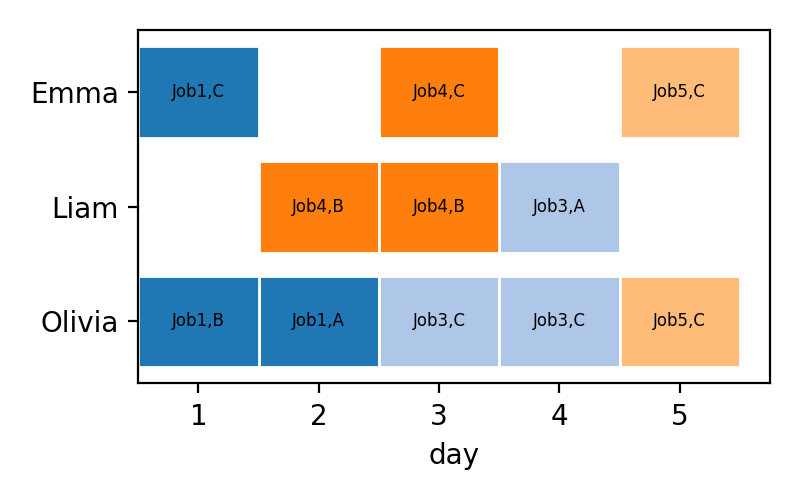
\includegraphics[width=\textwidth]{toy_schedule.png}\\[0.3em]
{\small Most profitable plan (65): Job2 skipped, all others on time.}
\end{columns}
\end{frame}

\begin{frame}{Results --- medium instance}
\centering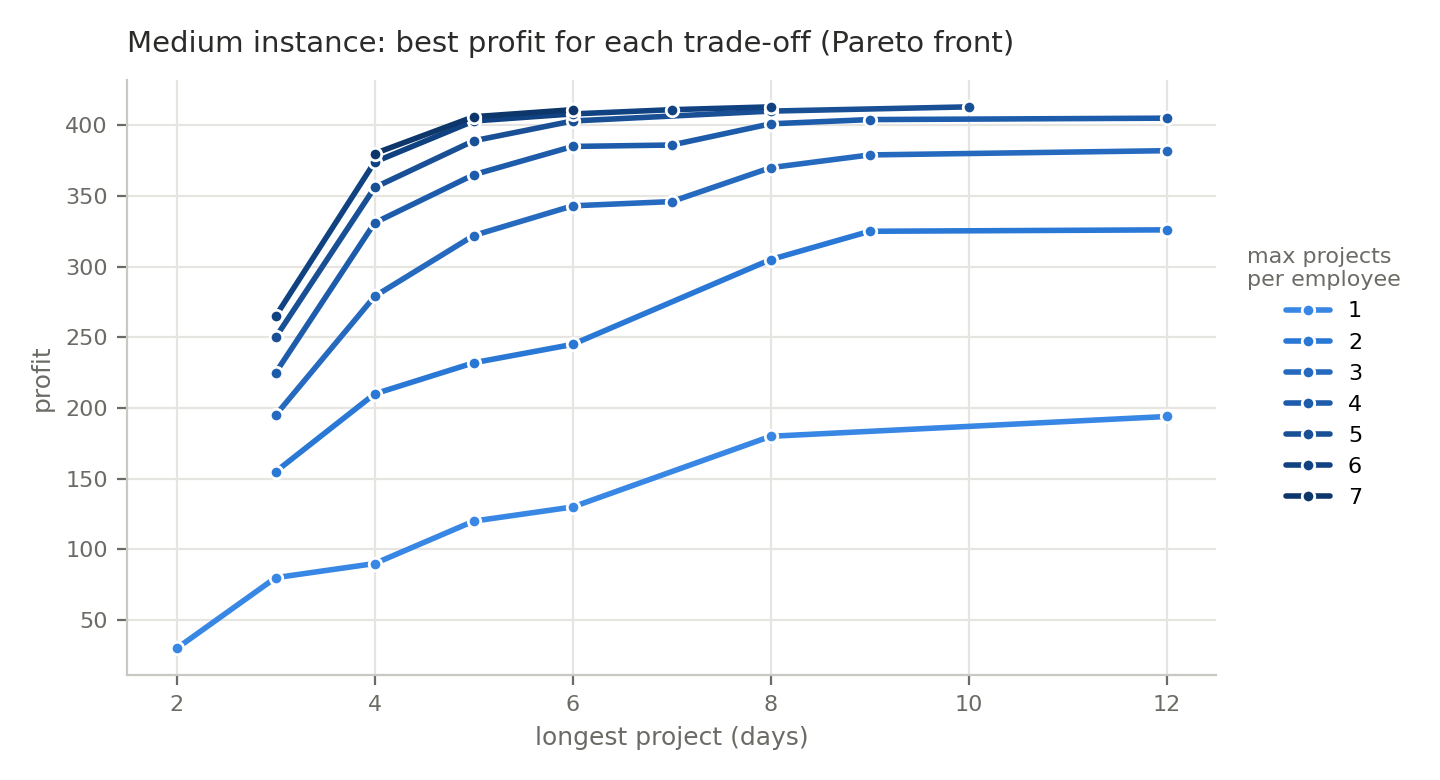
\includegraphics[height=0.66\textheight]{medium_front.png}\\
\small 413 is the maximum (P=6, D=8 or P=5, D=10); $-2\%$ allows 5-day projects or 4 projects per employee.
\end{frame}

\begin{frame}{Results --- medium schedule (profit 413)}
\centering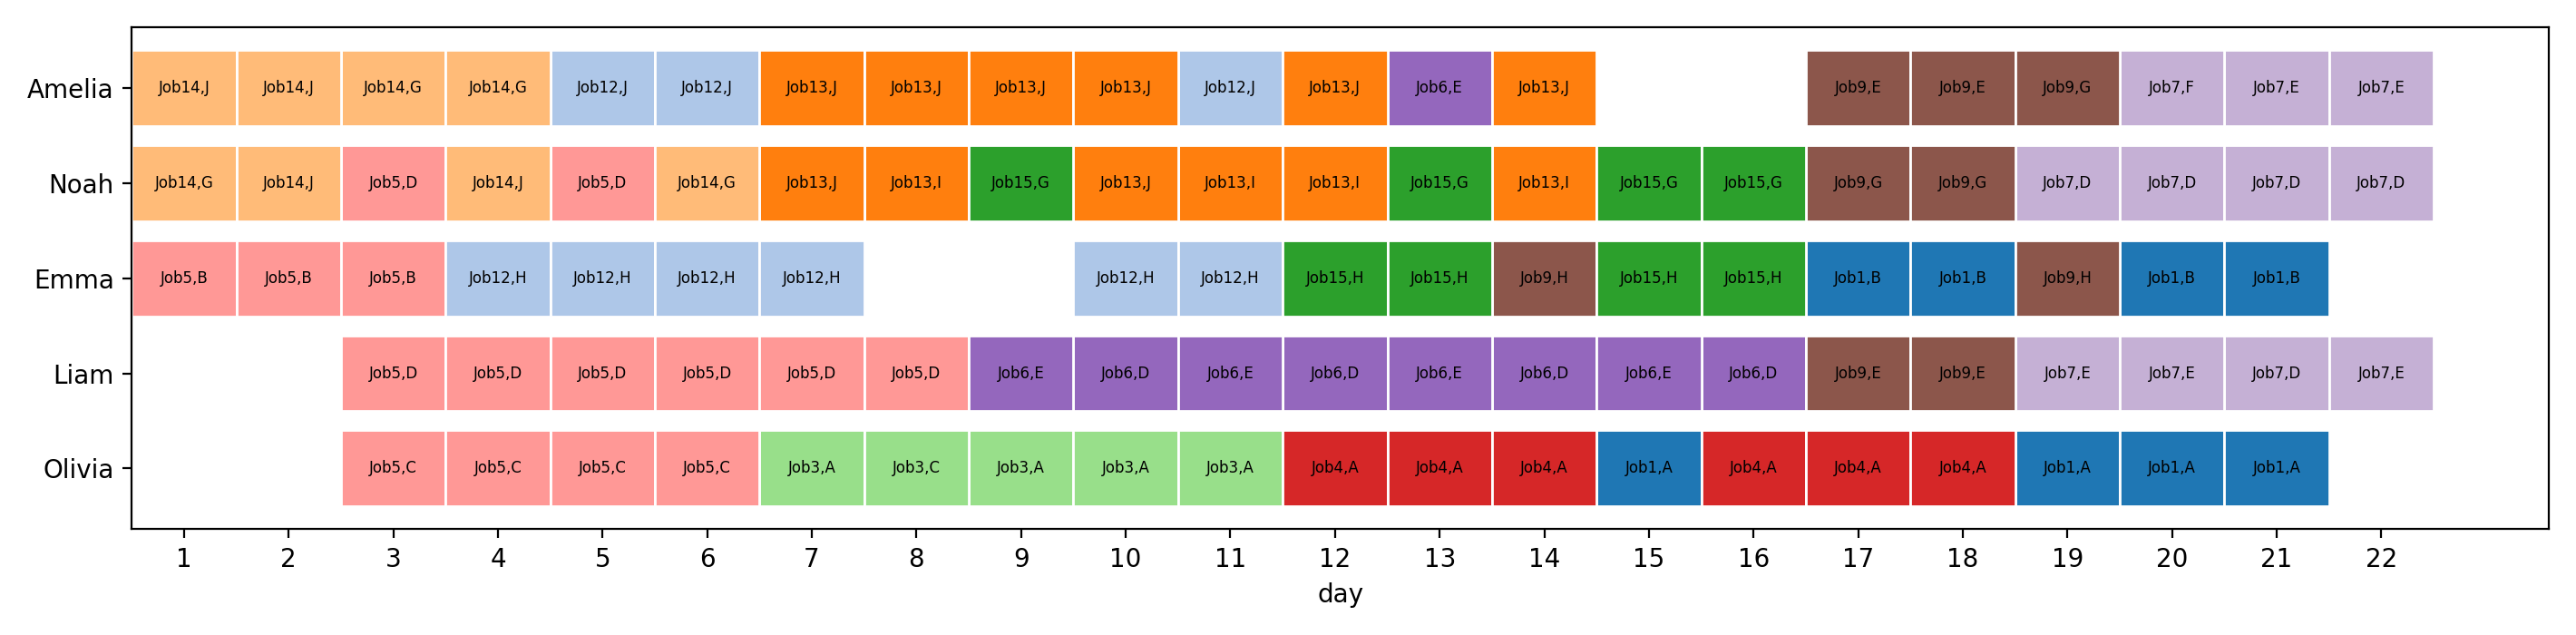
\includegraphics[width=\textwidth,height=0.75\textheight,keepaspectratio]{medium_schedule.png}
\end{frame}

\begin{frame}{Results --- large instance}
\begin{columns}[c]
\column{0.66\textwidth}
\centering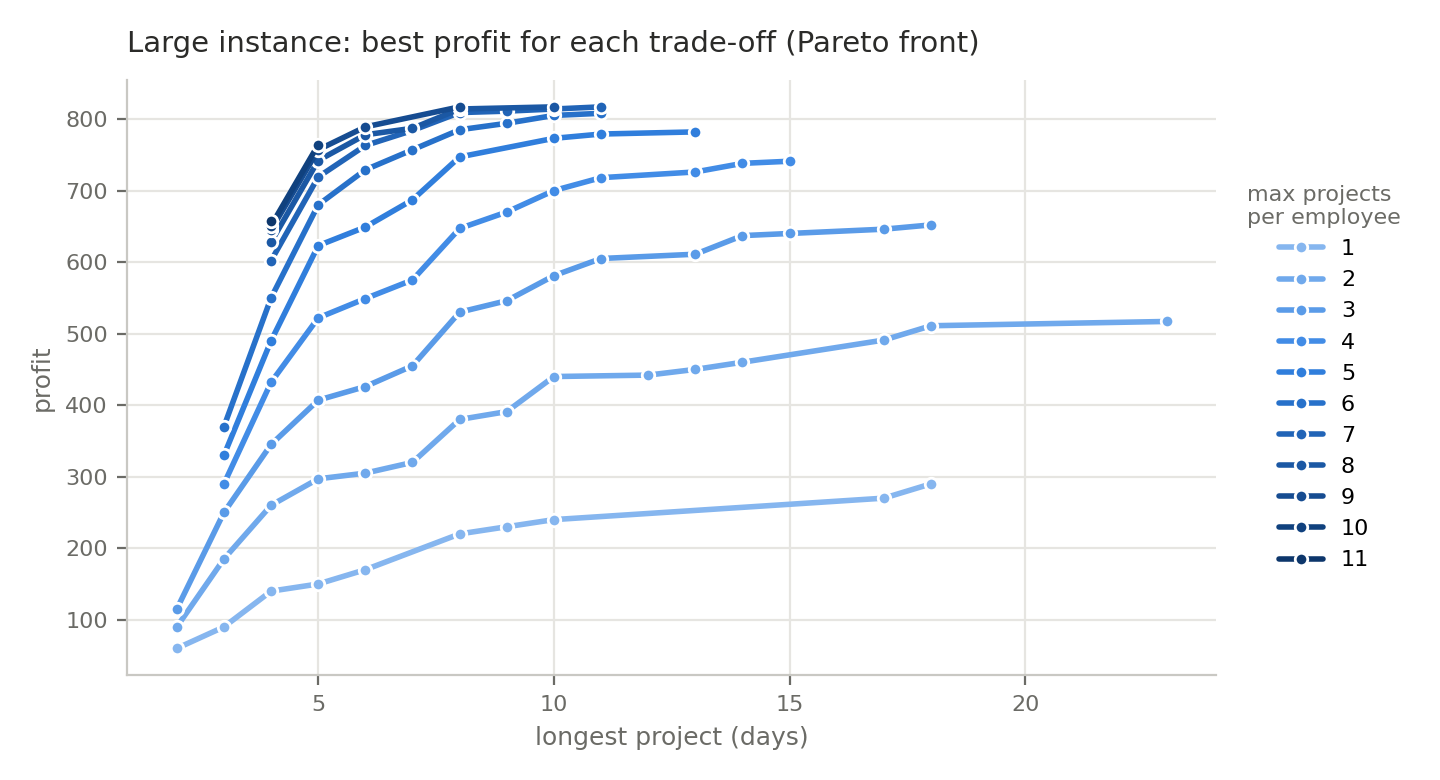
\includegraphics[width=\textwidth]{large_front.png}
\column{0.32\textwidth}
\small
\begin{tabular}{rcc}
\toprule
Profit & P & D\\
\midrule
817 & 9 & 8\\ 817 & 8 & 10\\ 817 & 7 & 11\\ 814 & 8 & 8\\ 811 & 7 & 9\\
808 & 6 & 11\\ 794 & 6 & 9\\ 782 & 5 & 13\\ 764 & 10 & 5\\
\bottomrule
\end{tabular}
\end{columns}
\vspace{0.4em}
\small $-3\%$ profit (794) cuts the workload from 9 to 6 projects per employee. Limits above 9 only help very short projects; above 11 nothing changes.
\end{frame}

\begin{frame}{Results --- large schedule (profit 817)}
\centering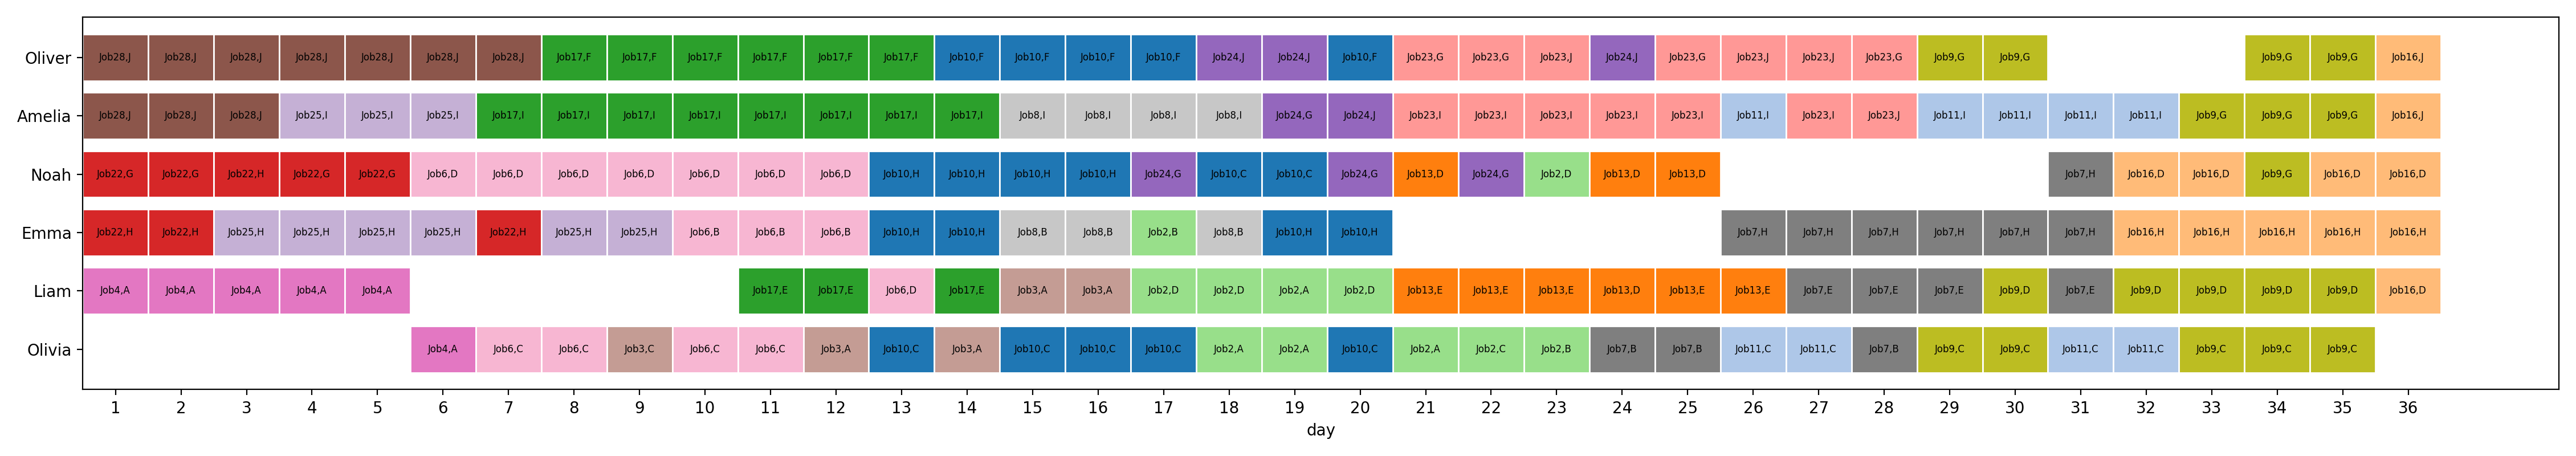
\includegraphics[width=\textwidth,height=0.75\textheight,keepaspectratio]{large_schedule.png}
\end{frame}

\begin{frame}{Instance generator}
\texttt{python generate\_instance.py out.json --staff 5 --jobs 12 --horizon 16 --quals 8 --seed 4}
\vspace{0.5em}
\begin{itemize}
  \item Each employee gets 1--5 random skills; every skill is held by at least one employee.
  \item Leave days: about 8\,\% of the horizon per employee (\texttt{--vacation}).
  \item Each project needs 1--4 skills; person-days are scaled so that total demand $\approx 1.3\times$ capacity (\texttt{--load}), as in the given instances: \alert{not every project can be done}.
  \item Gain $\approx 3.75$ per person-day $\pm 30\,\%$; due date between $h/3$ and $h$; penalty 3 per day late.
  \item Reproducible: same arguments and seed $\Rightarrow$ same file.
\end{itemize}
\end{frame}

\begin{frame}{Generated instances --- performance}
\centering\footnotesize
\begin{tabular}{lcccrrrrl}
\toprule
Instance & staff & projects & days & skills & solves & time & front & best (profit, P, D)\\
\midrule
toy (given) & 3 & 5 & 5 & 3 & 12 & 0.5 s & 9 & 65, 3, 2\\
gen1 & 3 & 6 & 8 & 4 & 21 & 1.7 s & 9 & 76, 4, 3\\
gen2 & 4 & 8 & 10 & 5 & 45 & 8.4 s & 17 & 103, 3, 5\\
gen3 & 4 & 10 & 14 & 6 & 73 & 90 s & 31 & 180, 5, 5\\
gen4 & 5 & 12 & 16 & 8 & 101 & 56 s & 28 & 222, 4, 8\\
medium (given) & 5 & 15 & 22 & 10 & 144 & 72 min & 46 & 413, 6, 8\\
large (given) & 6 & 25 & 36 & 10 & 347 & $\approx$35 h & 92 & 817, 9, 8\\
\bottomrule
\end{tabular}
\vspace{0.8em}
\begin{itemize}
  \item The number of solves grows roughly with projects $\times$ days; the time per solve grows much faster.
  \item Size alone does not decide difficulty: gen4 is bigger than gen3 but faster.
\end{itemize}
\end{frame}

\begin{frame}{Objective space and decision space (gen4)}
\begin{columns}[c]
\column{0.46\textwidth}
\centering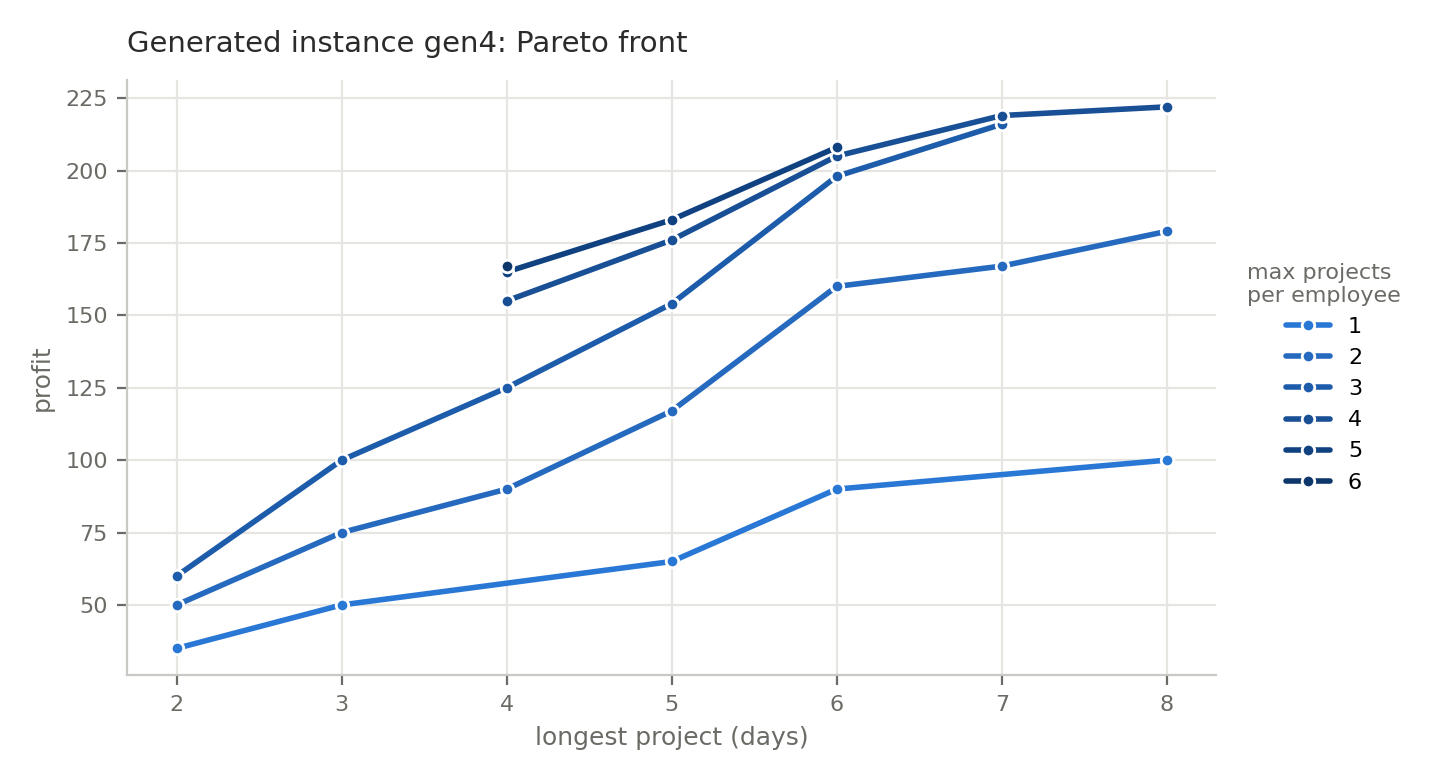
\includegraphics[width=0.9\textwidth]{generated/gen4_front.png}
\column{0.52\textwidth}
\small Any point of the front can be opened as a schedule:\\[0.3em]
{\footnotesize\texttt{python staffing.py gen4.json --plan 3 7}}\\[0.3em]
Below: profit 216 with at most 3 projects per employee and 7-day projects (the best plan earns 222 with 4 projects and 8-day projects).
\end{columns}
\vspace{0.2em}
\centering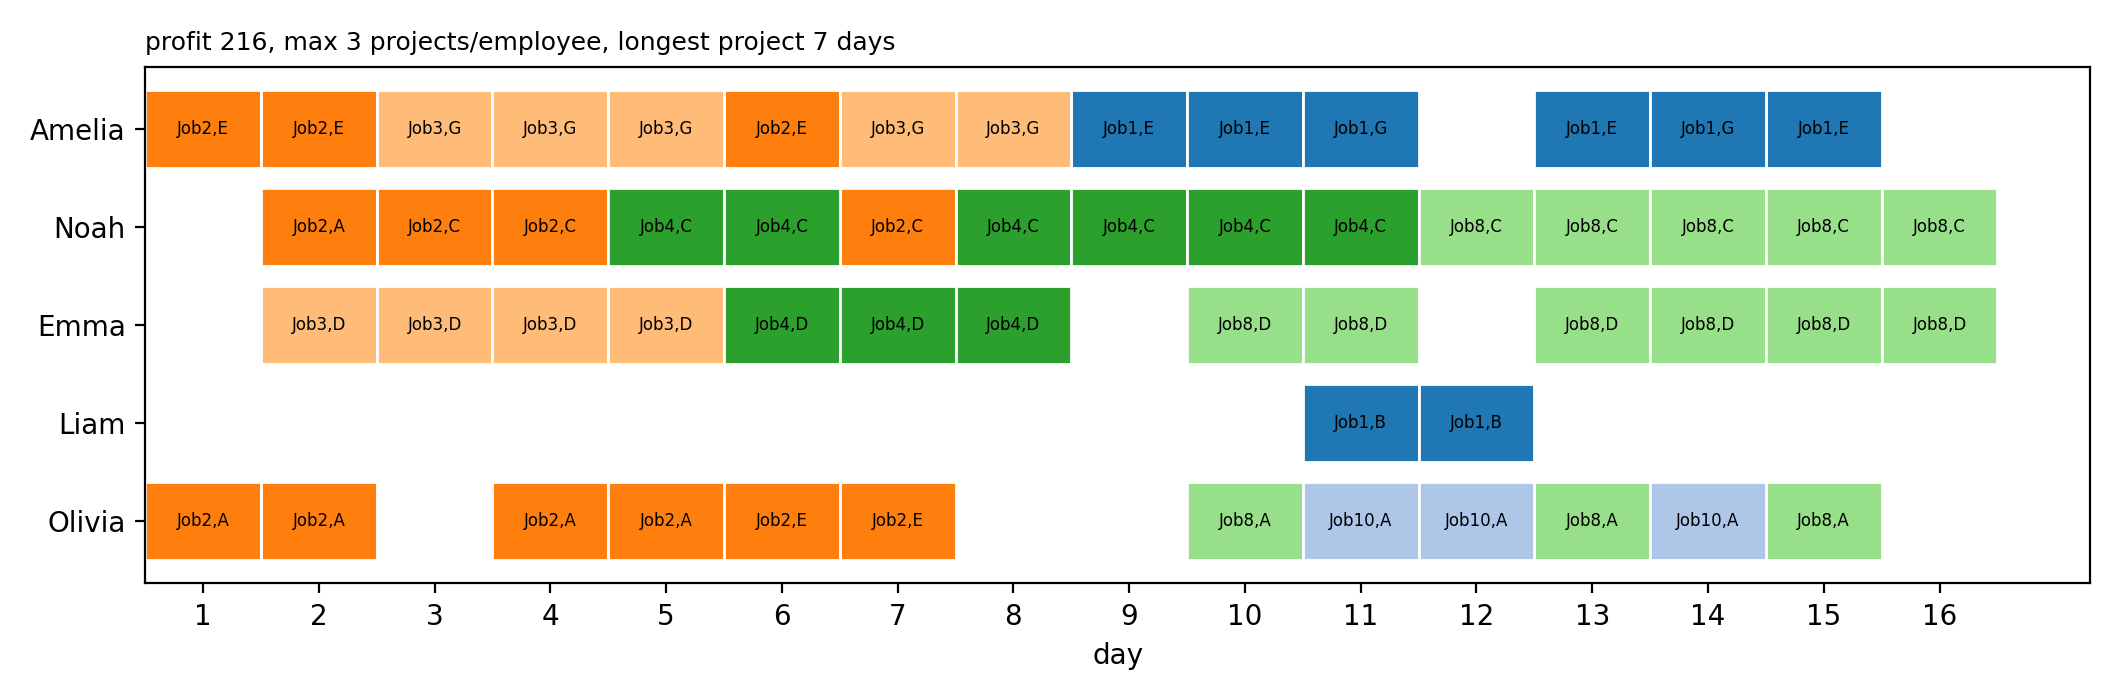
\includegraphics[width=0.72\textwidth]{generated/gen4_schedule_P3_D7.png}
\end{frame}

\begin{frame}{Conclusion}
\begin{itemize}
  \item Compact MILP solved \alert{exactly} with Gurobi on the three given instances and four generated ones.
  \item The $\varepsilon$-constraint method with the jump gives the complete Pareto front with far fewer solves (medium: 144 instead of 330).
  \item Formulation matters more than hardware: the time-window model made hard solves up to 28$\times$ faster.
  \item Look at sweet spots, not just the maximum: a few \% of profit buys much shorter projects or a lighter workload.
  \item Larger instances: time limit per solve, or stronger duration bounds.
\end{itemize}
\end{frame}
\end{document}
